\documentclass{standalone}
\usepackage{tikz}

\begin{document}
	\tikzset{
	font=\footnotesize,
	minimum width=20
		}
	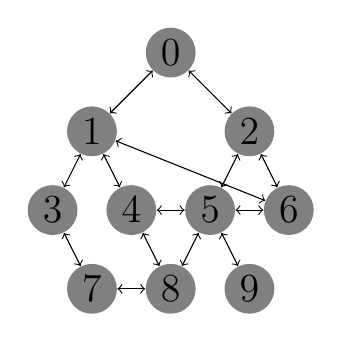
\begin{tikzpicture}
		\node[shape=circle,fill=gray, minimum size=18, inner sep=0.2pt] (a) at (10,0) {\Large{0}};
	%	\node[shape=circle,fill=gray] (h) at (10.75,0) {2};
		\node[shape=circle,fill=gray, minimum size=18, inner sep=0.2pt] (b) at (9,-1) {\Large{1}};
		\node[shape=circle,fill=gray, minimum size=18, inner sep=0.2pt] (c) at (11,-1) {\Large{2}};
		\node[shape=circle,fill=gray, minimum size=18, inner sep=0.2pt] (d) at (8.5,-2) {\Large{3}};
		\node[shape=circle,fill=gray, minimum size=18, inner sep=0.2pt] (e) at (9.5,-2) {\Large{4}};
		\node[shape=circle,fill=gray, minimum size=18, inner sep=0.2pt] (f) at (10.5,-2) {\Large{5}};
		\node[shape=circle,fill=gray, minimum size=18, inner sep=0.2pt] (g) at (11.5,-2) {\Large{6}};
		\node[shape=circle,fill=gray, minimum size=18, inner sep=0.2pt] (x) at (9,-3) {\Large{7}};
		\node[shape=circle,fill=gray, minimum size=18, inner sep=0.2pt] (y) at (10,-3) {\Large{8}};
		\node[shape=circle,fill=gray, minimum size=18, inner sep=0.2pt] (z) at (11,-3) {\Large{9}};
		\draw (a) edge[<->] (b) (a) edge[<->] (c) 	
	%	(h) edge[<->] (c)
		(b) edge[<->] (d)  (b) edge[<->] (g)
		(c) edge[<->] (f) (c) edge[<->] (g)
		(b) edge[<->] (e) (e) edge[<->] (f) (f) edge[<->] (g)
		(d) edge[<->] (x) (e) edge[<->] (y) (f) edge[<->] (z) (f) edge[<->] (y)
		(x) edge[<->] (y); 
	\end{tikzpicture}
\end{document}  